% Tecnología elegida (JADE)

\chapter*{Tecnología elegida} \label{cap4}
\addcontentsline{toc}{chapter}{Tecnología elegida}

\begin{flushright}
\begin{minipage}{7.85cm}
    {\em Cualquier tecnología lo suficientemente avanzada es indistinguible de
    la magia.} \\ Arthur C. Clarke
\end{minipage}
\end{flushright}

\vspace*{5mm}

\section*{Licencias}

Para este proyecto vamos a usar la licencia GPL (Licencia Pública General de
GNU) en su versión 3 o posterior, escrita y mantenida por la FSF\footnote{Free
Software Foundation: \url{http://www.fsf.org/}}. El texto legal se puede
encontrar en el \hyperref[ap1]{Apéndice primero}.

Al colocar el simulador bajo esta licencia nos tenemos que asegurar que todas
las librerías que utilicemos estén bajo licencias compatibles con la nuestra. A
continuación sigue un gráfico con la relación de compatibilidad de otras
licencias libres con la GPL v3.

\begin{figure}[H]
 \centering
 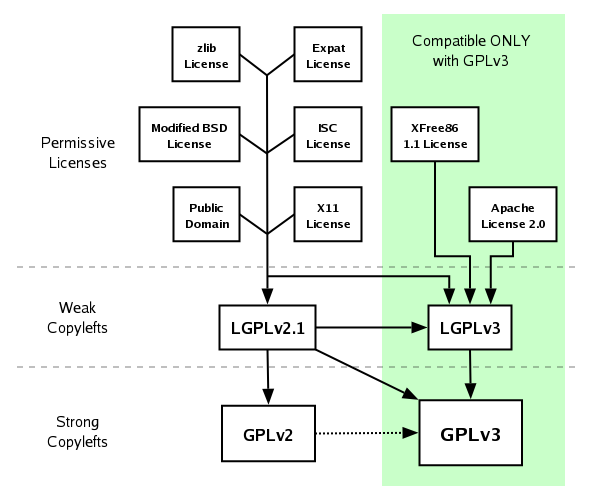
\includegraphics[width=120mm]{figuras/cap4/gplv3_comp.png}
 \caption{Compatibilidad de otras licencias libres con la GPL v3}
\end{figure}

\section*{JADE}

La plataforma JADE (Java Agent DEvelopment Framework) es la escogida para el
desarrollo del simulador. El objetivo principal de esta plataforma es la
simplificación del desarrollo de sistemas multiagentes, siguiendo a su vez los
estándares de comunicación entre sistemas de la FIPA\footnote{Foundation for
Intelligent Physical Agents: \url{http://www.fipa.org/}}.

\begin{figure}[H]
 \centering
 
\includegraphics[width=30mm]{figuras/cap4/jade.png}
 \caption{Logo de JADE}
\end{figure}

Al utilizar JADE el desarrollador sólo tiene que concentrarse en los agentes
que escriba, el resto de aspectos del sistema están ya resueltos, tales como el
intercambio de mensajes, la búsqueda de agentes, el ciclo de vida de estos,
etc. Además está escrita en Java, lo que aumenta la portabilidad a múltiples
entornos de ejecución frente otros lenguajes de programación.

El hecho de utilizar JADE nos condiciona a utilizar Java como lenguaje y
plataforma de desarrollo para el proyecto. El resto de librerías y paquetes que
utilizamos, y que describimos en los siguientes apartados, están pues escritos
en este lenguaje.

Dado que nuestro proyecto hace uso de la licencia \hyperref[ap1]{GPL v3}, es
vital que el software que utilicemos sea también libre y esté bajo una licencia
compatible. En concreto JADE usa la licencia LGPL\footnote{Licencia Pública
General Reducida de GNU:
\url{http://www.gnu.org/licenses/old-licenses/lgpl-2.0.html}} v2.

Además de ser Software Libre, JADE tiene también la virtud de cumplir con la
especificación completa de la FIPA. Cumplir con dichos estándares es muy
importante para que sea posible la interacción entre sistemas multiagentes, y
que el proyecto no sea un entorno cerrado sin capacidad de comunicación.

JADE está desarrollado y mantenido por Telecom
Italia\footnote{\url{http://jade.tilab.com/}}.

\section*{Java}

Java es un lenguaje de programación orientado a objetos desarrollado por Sun
Microsystems, recientemente adquirida por Oracle, a principios de los años 90.
El leitmotiv de los desarrolladores de Java era {\em write once, run anywhere},
que hace referencia a la portabilidad de un programa Java, capaz de ejecutarse
allá donde hubiera una máquina virtual, una de las características más notorias
de la plataforma.

La elección de utilizar Java viene condicionada a la elección de utilizar JADE,
que está escrito en este lenguaje.

De Java existe una implementación totalmente libre de nombre
OpenJDK\footnote{\url{http://openjdk.java.net/}}. OpenJDK soporta el 99\% de la
plataforma, y el simulador podrá ejecutarse sobre esta implementación.

\section*{JAK}

JAK (Java API for KML) son un conjunto de librerías para el manejo de ficheros
KML desde Java. JAK ha sido desarrollado por Micromata
GmbH\footnote{\url{http://labs.micromata.de/display/jak/Home}}.

\begin{figure}[H]
 \centering
 
\includegraphics[width=30mm]{figuras/cap4/jak.png}
 \caption{Logo de JAK}
\end{figure}

Al igual que en el caso de {\bf JADE} es necesario que JAK sea compatible con
la licencia de nuestro proyecto, la \hyperref[ap1]{GPL v3}.
Los desarrolladores de JAK optaron por liberar las librerías bajo una licencia
BSD\footnote{Berkeley Software Distribution:
\url{http://www.opensource.org/licenses/bsd-license.php}} de 3 clausulas, o como
también se la conoce, licencia BSD modificada o nueva licencia BSD. La licencia
de JAK se puede consultar en su sitio web.

Gracias a JAK podremos generar los ficheros KML con el resultado de la
simulación.

\section*{Jcoord}

Para el manejo de coordenadas geográficas utilizaremos
Jcoord\footnote{\url{http://www.jstott.me.uk/jcoord/}}, un paquete de clases que
nos permitirán convertir entre formatos de coordenadas, calcular distancias,
etc. Jcoord ha sido desarrollado por Jonathan Mark Stott, y tal como se puede
consultar en su sitio web está licenciado bajo GPL v2, compatible con nuestra
\hyperref[ap1]{GPL v3}.

Además del habitual sistema de coordenadas latitud/longitud
WGS84\footnote{Sistema Geodésico Mundial 1984} soporta UTM\footnote{Sistema de
Coordenadas Universal Transversal de Mercator}.

A diferencia de {\bf JADE} o {\bf JAK}, integraremos directamente el código en
el simulador, por lo que no será una dependencia. De esta manera podremos
modificar y adaptar el paquete a nuestras necesidades.

\section*{Otras librerías}

\subsection*{Java CSV}

Java CSV\footnote{\url{http://sourceforge.net/projects/javacsv/}} es una
sencilla librería que facilita la escritura y lectura de ficheros de valores
separados por coma. Lo utilizaremos para escribir en ficheros los datos del
módulo de estadísticas.

La licencia de esta librería es la LGPL v2.1 o posterior, y estará integrada en
el código del proyecto por lo que no será una dependencia.

\subsection*{OpenWFE}

Del proyecto OpenWFE\footnote{Open WorkFlow Engine:
\url{http://sourceforge.net/projects/openwfe/}} en realidad sólo utilizaremos
una clase. Una implementación de Wget en Java (una herramienta para descargar
ficheros de la web). La licencia de OpenWFE es una BSD de 3 clausulas.

Dicha clase estará integrada en el código del simulador por lo que OpenWFE no
será una dependencia.

\section*{Servicios}

Además de las librerías comentadas hasta ahora haremos uso de algunos
servicios, como son Open Street Maps y el servicio web de elevaciones de la
USGS descritos en \hyperref[cap3]{el capítulo 3}.

\subsection*{Open Street Maps}

Open Street Maps (OSM)\cite{Pinto09} permite que se le realicen peticiones GET
por HTML, y
devuelve directamente un fichero con la información solicitada en
XML\footnote{Lenguaje de Marcado Extensible: \url{http://www.w3.org/XML/}}. La
implementación de la petición será por lo tanto sencilla, aunque el tratamiento
de los datos recibidos requerirá de un procesado mucho más complejo.

\begin{figure}[H]
 \centering
 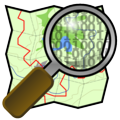
\includegraphics[width=20mm]{figuras/cap4/osm.png}
 \caption{Logo de Open Street Maps}
\end{figure}

\subsection*{Servicio de elevaciones de la USGS}

La U.S. Geological Survey (USGS) proporciona un método para obtener la elevación
del terreno si éste pertenece a los Estados Unidos. Este servicio consiste en un
servicio web al que se accede a través de SOAP\footnote{Simple Object Access
Protocol: \url{http://www.w3.org/TR/soap/}}. Para consumir dicho servicio hace
falta implementar un cliente, tarea que gracias a Java resulta bastante
sencilla.

Utilizaremos la herramienta {\bf wsimport} que trae Java para autogenerar el
código del cliente del servicio web, código que irá incluido en el proyecto.

\begin{figure}[H]
 \centering
 
\includegraphics[width=35mm]{figuras/cap4/usgs.png}
 \caption{Logo de la USGS}
\end{figure}

%%% Local Variables:
%%% mode: latex
%%% TeX-master: "../dissim"
%%% End: